\documentclass[ignorenonframetext,plain,fleqn]{beamer}
\setbeamertemplate{navigation symbols}{}

\usepackage{verbatim}
\newcommand{\vocab}{\mathcal{V}}
\newcommand{\corpus}{\mathcal{C}}
\newcommand{\pml}{p_{\textsc{ml}}}
\DeclareMathOperator*{\argmax}{argmax}
\DeclareMathOperator*{\argmin}{argmin}
\newcommand{\score}{\mathit{score}}
\newcommand{\loss}{\mathit{loss}}
\renewcommand{\vec}{\mathbf}
\newcommand{\pluseq}{\mathrel{+}=}
\newcommand{\sos}{\mbox{$\langle$s$\rangle$}}
\newcommand{\eos}{\mbox{$\langle/$s$\rangle$}}

\title{Learning to map strings to trees}
\subtitle{Comp 542 Natural Language Processing}
\author{Deniz Yuret}

\hypersetup{colorlinks,urlcolor=red}

\begin{document}

\begin{frame}
\maketitle
\end{frame}

%\section{Generative models}
%\frame{\sectionpage}

\begin{frame}\frametitle{Phrase structure trees (Figure from LSP)}
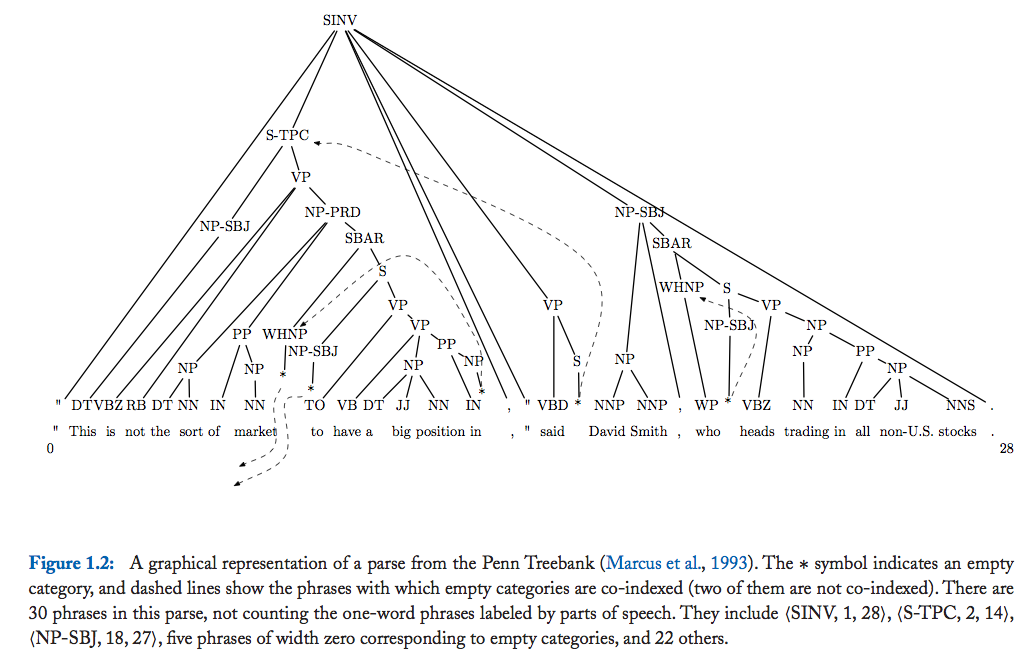
\includegraphics[width=\textwidth]{images/smith-fig-1-2.png}
\end{frame}

\begin{frame}[fragile]\frametitle{Penn Treebank representation}
\begin{tiny}
\verbatiminput{images/pstree.txt}
\end{tiny}
\end{frame}

\begin{frame}\frametitle{Hidden Markov Models: Generative Process}
To generate each $(\vec{x},\vec{y})$ pair where $\vec{x} = (x_1, x_2,
\dots, x_n)$ consists of words $x_i$ from a vocabulary $\Sigma$ and
$\vec{y} = (y_1, y_2, \dots, y_n)$ consists of tags $y_i$ from a tag
set $\Lambda$:
\begin{itemize}
\item Generate a start symbol $y_0=\sos$.
\item For $i=1, 2, \dots$:
\begin{itemize}
\item Transition: sample $y_i$ from $p(y_i|y_{i-1})$.
\item Return $(\vec{x}, \vec{y})$ if $y_i=\eos$.
\item Emission: sample $x_i$ from $p(x_i|y_i)$.
\end{itemize}
\end{itemize}
\end{frame}

\end{document}
